

\chapter{TINJAUAN PUSTAKA}
\label{cha:2-TinjauanPustaka}

\section{Teorema Penaksiran Universal}
\label{sec:2-TeoremaPenaksiranUniversal}

Teorema penaksiran universal atau \textit{universal approximation theorem} menyatakan bahwa sebuah
model jaringan \textit{feed-forward} dapat membentuk fungsi apapun secara subjektif. Sebuah model
jaringan saraf tiruan dibentuk dari serangkaian lapisan yang didalamnya terdapat deretan sel saraf
atau \textit{neuron} dengan kuantitas tertentu. Semakin panjang rangkaian lapisan yang tersedia,
maka semakin banyak saraf yang tersedia sehingga dapat memetakan fungsi yang sulit.
Model jaringan yang memiliki banyak saraf dapat mempelajari pola-pola yang ada dari satu
domain ke domain lainnya~\cite{2016arXiv160100013G}.

Teorema penaksiran universal memiliki dua sifat yang dikategorikan berdasarkan pemanfaatannya dalam
melakukan pemelajaran mesin. Sifat pertama adalah suatu model jaringan saraf tiruan dapat
memperkirakan suatu fungsi dengan batasan-batasan tertentu sesuai dengan fungsi keluaran pada setiap
lapisan yang terdapat dalam model khususnya lapisan yang terdapat pada bagian akhir.
Sifat kedua adalah sebuah fungsi kontinu dengan jumlah variabel sembarang dapat
ditiru sifatnya oleh sebuah jaringan saraf tiruan dengan jumlah parameter yang sembarang~\cite{2019arXiv191003344K}.

\begin{figure}[htbp]
    \begin{center}
        \fbox{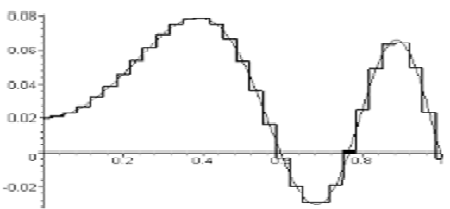
\includegraphics[scale=1.0]{bab2/gambar/uat.png}}
    \end{center}
    \vspace{-20pt}
    \captionsetup{labelfont=bf, textfont=bf}
    \caption{Teorema Penaksiran Universal}
    \vspace{-10pt}
    \captionsetup{labelfont=md, textfont=md}
    \caption*{Sumber: https://encrypted-tbn0.gstatic.com/images?q=tbn}
    % \caption*{Sumber: Zhang (2019)}
    \label{fig:uat}
\end{figure}

\section{Jaringan Saraf}
\label{sec:2-JaringanSaraf}

Otak manusia terdiri dari kumpulan sel saraf yang saling terkoneksi satu sama lain. Sebuah sel saraf
adalah sel yang dapat memproses dan mengantarkan informasi apabila dirangsang dengan tegangan
elektrokimia. Sel-sel saraf tidak membelah dirinya dan tidak digantikan apabila ada yang
rusak. Jumlah sel saraf yang terdapat dalam otak manusia diperkirakan sebanyak satu miliar. Setiap
sel saraf diperkirakan berkoneksi dengan sepuluh ribu sel saraf lainnya melalui sinapsis yang
berarti otak manusia dewasa beroperasi seperti prosesor dengan kecepatan satu triliun bit per
detik~\cite{10.3389/neuro.09.031.2009}.

\begin{figure}[htbp]
    \begin{center}
        \fbox{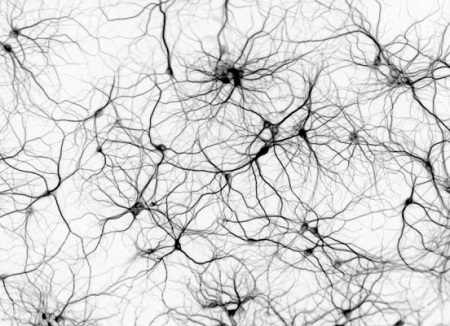
\includegraphics[scale=1.0]{bab2/gambar/jaringansaraf.jpg}}
    \end{center}
    \vspace{-20pt}
    \captionsetup{labelfont=bf, textfont=bf}
    \caption{Ilustrasi Jaringan Saraf Manusia}
    \vspace{-10pt}
    \captionsetup{labelfont=md, textfont=md}
    \caption*{Sumber: https://wccftech.com/scientists-artificial-neurons}
    % \caption*{Sumber: Zhang (2019)}
    \label{fig:jaringansaraf}
\end{figure}

Bentuk sel saraf sangat bervariasi dengan berbagai ukuran, bentuk, dan sifat elektrokimianya. Sebuah
sel saraf memiliki badan yang terdiri dari beberapa struktur penting meliputi \textit{soma},
\textit{dendrites}, \textit{axon}, dan \textit{synapses} seperti pada gambar~\ref{fig:selsaraf}.
Sebuah sel saraf akan menerima beberapa masukkan melalui \textit{synapses}, memproses inputan
tersebut melewati \textit{dendrites}, kemudian diteruskan melalui \textit{soma}, dan diberikan
kepada sel saraf lainnya melalui \textit{axon}~\cite{2019arXiv190601703Z}.

\begin{figure}[htbp]
    \begin{center}
        \fbox{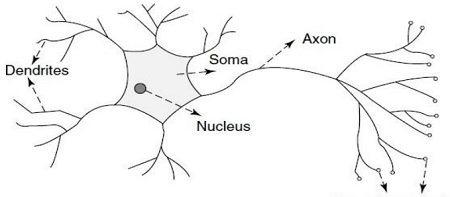
\includegraphics[scale=1.0]{bab2/gambar/selsaraf.jpg}}
    \end{center}
    \vspace{-20pt}
    \captionsetup{labelfont=bf, textfont=bf}
    \caption{Ilustrasi Sel Saraf Manusia}
    \vspace{-10pt}
    \captionsetup{labelfont=md, textfont=md}
    \caption*{Sumber: https://en.wikipedia.org/wiki/Neuron}
    % \caption*{Sumber: Zhang (2019)}
    \label{fig:selsaraf}
\end{figure}

\pagebreak

\section{Jaringan Saraf Tiruan}
\label{sec:2-JaringanSarafTiruan}

Jaringan Saraf Tiruan adalah sistem komputasi yang cara kerjanya menyerupai jaringan saraf pada otak
makhluk hidup. Sebuah jaringan saraf tiruan dapat dengan mandiri
memodelkan fungsi sembarang yang tingkat kesulitannya sesuai dengan jumlah koneksi yang tesedia.
Jarigan ini menyerupai jaringan saraf asli dimana
sebuah saraf tiruan menerima banyak masukkan dari saraf lainnya
kemudian dioperasikan dengan bobot yang terkadung pada sel tersebut dan akhirnya diteruskan ke sel
berikutnya~\cite{Sharma2012ACS}.

Sebuah sel saraf dapat dibagi menjadi empat bagian yang meliputi masukkan, bobot, fungsi
transfer atau aktivasi, dan keluaran. Jumlah masukkan pada suatu sel saraf tiruan berjumlah sebanyak
output dari sel-sel yang berada pada layer sebelumnya. Bobot sel adalah nilai numerik yang menjadi
identitas dari sel yang merupakan hasil penyesuaian dari proses latihan. Fungsi aktivasi adalah
sebuah fungsi menerima hasil operasi antara bobot dan masukkan. Keluaran merupakan hasil dari sel
yang diteruskan ke lapisan selanjutnya. Ilustrasi sebuah sel saraf tiruan dapat dilihat pada gambar
~\ref{fig:saraftiruan}~\cite{Sharma2012ACS}.

\begin{figure}[htbp]
    \begin{center}
        \fbox{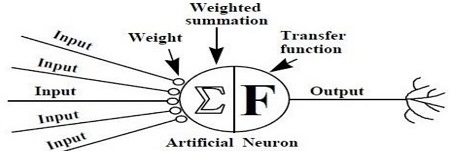
\includegraphics[scale=1.0]{bab2/gambar/saraftiruan.jpg}}
    \end{center}
    \vspace{-20pt}
    \captionsetup{labelfont=bf, textfont=bf}
    \caption{Ilustrasi Sel Saraf Tiruan}
    \vspace{-10pt}
    \captionsetup{labelfont=md, textfont=md}
    \caption*{Sumber: https://en.wikipedia.org/wiki/artificial\_neural\_network}
    % \caption*{Sumber: Zhang (2019)}
    \label{fig:saraftiruan}
\end{figure}

\pagebreak

\section{Fungsi Aktivasi}
\label{sec:2-FungsiAktivasi}

Fungsi aktivasi pada sel saraf tiruan berfungsi untuk mengkonversi hasil operasi matriks antara
masukkan dan bobot sebuah sel dari sistem linier menjadi sistem nonlinier. Konversi nilai ini dilakukan
agar setiap sel mengambil perannya pada saat proses pelatihan model. Beberapa fungsi aktivasi yang
dipakai pada umumnya adalah \textit{Sigmoid}, \textit{ReLU}, \textit{Tanh}, dan \textit{Softmax}
~\cite{2014arXiv1412.6830A}.

\textit{Rectified Linear Unit} adalah fungsi aktivasi yang paling umum digunakan dalam aplikasi
jaringan saraf tiruan. Fungsi aktivasi \textit{ReLU} membatasi nilai masukkannya dimana nilai yang
kurang dari nol akan diubah menjadi nol~\cite{Hinton_rectifiedlinear, 2018arXiv181103378N}.
Fungsi aktivasi \textit{Rectified Linear Unit} dapat dilihat pada persamaan 2.1 dengan grafik yang
dapat dilihat pada gambar~\ref{fig:relu}.

\begin{equation}
    \;f(x)=\;max\left(0,x\right)=\;\left\{\begin{array}{l}x_{i,\;}\;\;if\;x_i\;\geq\;0\\0,\;\;\;\;if\;x_i<\;0\;\;\end{array}\right.\;\;
\end{equation}

\begin{figure}[htbp]
    \begin{center}
        \fbox{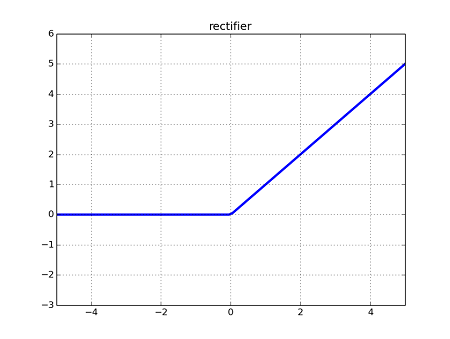
\includegraphics[scale=1.0]{bab2/gambar/relu.png}}
    \end{center}
    \vspace{-20pt}
    \captionsetup{labelfont=bf, textfont=bf}
    \caption{\textit{Rectified Linear Unit}}
    \vspace{-10pt}
    \captionsetup{labelfont=md, textfont=md}
    \caption*{Sumber: https://static.packt-cdn.com/products/graphics/B05478\_03\_11.png}
    % \caption*{Sumber: Zhang (2019)}
    \label{fig:relu}
\end{figure}

\section{\textit{Residual Network}}
\label{sec:2-ResidualNetwork}

\textit{Residual Network} atau \textit{ResNet} merupakan model jaringan saraf tiruan yang menggunakan \textit{residual block}
sebagai dasar dari setiap lapisan. Sebuah \textit{residual block} merupakan sebuah arsitektur jaringan
saraf tiruan kecil yang terdiri dari beberapa lapisan. Setiap blok akan menjumlahkan masukkan dan
keluarannya sehingga layer di dalam suatu blok hanya menambahkan pola-pola yang dipelajari.

Hal ini
memungkinkan \textit{ResNet} untuk memiliki jumlah blok yang sangat banyak sehingga dapat memetakan
suatu fungsi sembarang yang sulit sesuai dengan teorema penaksiran universal~\cite{2015arXiv151203385H}.
Jenis-jenis \textit{residual block} dapat dilihat pada gambar~\ref{fig:resblock}.

\begin{figure}[htbp]
    \begin{center}
        \fbox{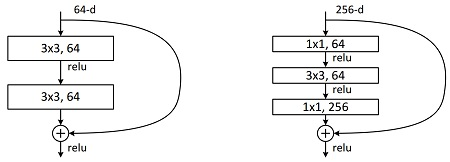
\includegraphics[scale=1.0]{bab2/gambar/resnet.jpg}}
    \end{center}
    \vspace{-20pt}
    \captionsetup{labelfont=bf, textfont=bf}
    \caption{\textit{Residual Block}}
    \vspace{-10pt}
    \captionsetup{labelfont=md, textfont=md}
    \caption*{Sumber: https://arxiv.org/abs/1512.03385}
    % \caption*{Sumber: Zhang (2019)}
    \label{fig:resblock}
\end{figure}

\section{Optimisasi Model}
\label{sec:2-OptimisasiModel}

Algoritma optimisasi model yang paling populer dalam melakukan pemelajaran model \textit{deep learning}
adalah \textit{gradient descent}. \textit{Gradient descent} meminimalisir selisih antara prediksi
model dan target sebenarnya dengan merubah bobot-bobot yang terdapat dalam model. Nilai bobot yang
ditambahkan berbanding terbalik dengan gradien hasil fungsi kesalahan terhadap masing-masing bobot.
Proses optimisasi dilakukan dengan melakukan \textit{backpropagation} yang
melibatkan beberapa elemen seperti \textit{learning rate},
dan \textit{loss function}. Tujuannya adalah untuk mencapai titik optimal pada sebuah bidang berdasarkan
hasil dari \textit{loss function}~\cite{2016arXiv160100013G}. Ilustrasi titik optimal digambarkan
pada gambar~\ref{fig:gradientdescent}.

\begin{figure}[htbp]
    \begin{center}
        \fbox{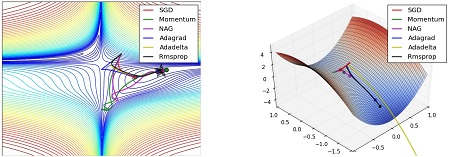
\includegraphics[scale=1.0]{bab2/gambar/gradientdescent.jpg}}
    \end{center}
    \vspace{-20pt}
    \captionsetup{labelfont=bf, textfont=bf}
    \caption{\textit{Gradient Descent}}
    \vspace{-10pt}
    \captionsetup{labelfont=md, textfont=md}
    \caption*{Sumber: https://arxiv.org/abs/1601.00013}
    % \caption*{Sumber: Zhang (2019)}
    \label{fig:gradientdescent}
\end{figure}

\subsection{\textit{Backpropagation}}

\textit{Backpropagation} adalah sebuah prosedur pemelajaran jaringan saraf tiruan yang secara
berulang-ulang kali menyesuaikan bobot setiap sel hingga selisih antara keluaran dan target menjadi
lebih kecil. Algoritma ini merupakan mengorganisasikan sebuah model jaringan untuk secara mandiri
mencari titik optimal secara berkala. Optimisasi dilakukan dengan melakukan \textit{forward-pass}
pada satu atau sebagian atau semua data yang ada ke dalam model untuk mendapatkan hasil prediksi.
Hasil tersebut kemudian diukur selisihnya dengan target yang sebenarnya menggunakan sebuah fungsi
kesalahan. Turuan parsial masing-masing bobot terhadap selisih kesalahan ini adalah kuantitas negatif
yang harus ditambahkan bobot yang berkaitan~\cite{Rumelhart:1986we}. Skema algoritma \textit{backpropagation}
dapat dilihat pada gambar~\ref{fig:backprop}.

\begin{figure}[htbp]
    \begin{center}
        \fbox{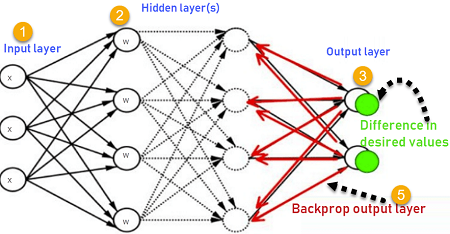
\includegraphics[scale=1.0]{bab2/gambar/backprop.png}}
    \end{center}
    \vspace{-20pt}
    \captionsetup{labelfont=bf, textfont=bf}
    \caption{Skema \textit{Backpropagation}}
    \vspace{-10pt}
    \captionsetup{labelfont=md, textfont=md}
    \caption*{Sumber: https://www.nature.com/articles/323533a0}
    % \caption*{Sumber: Zhang (2019)}
    \label{fig:backprop}
\end{figure}

\pagebreak

\subsection{\textit{Learning Rate}}

\textit{Learning rate} adalah sebuah nilai skalar yang menentukan seberapa besar sebuah bobot pada
jaringan saraf akan ditambahkan. Nilai \textit{learning rate} umumnya bernilai kecil karena
besar turunan parsial pada setiap iterasi akan berubah-ubah. Nilai \textit{learning rate} yang besar
akan merubah bobot dengan skala yang besar sehingga akurasi model cederung tidak stabil. Nilai
\textit{learning rate} yang kecil akan menghasilkan model yang stabil tetapi memerlukan jumlah iterasi
yang banyak seperti pada gambar~\ref{fig:lr}~\cite{2019arXiv190801878Y}.

\begin{figure}[htbp]
    \begin{center}
        \fbox{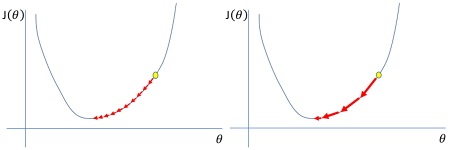
\includegraphics[scale=1.0]{bab2/gambar/lr.jpg}}
    \end{center}
    \vspace{-20pt}
    \captionsetup{labelfont=bf, textfont=bf}
    \caption{Ilustrasi Perbedaan \textit{Learning Rate}}
    \vspace{-10pt}
    \captionsetup{labelfont=md, textfont=md}
    \caption*{Sumber: https://arxiv.org/abs/1908.01878}
    % \caption*{Sumber: Zhang (2019)}
    \label{fig:lr}
\end{figure}

\subsection{\textit{Mean Squared Error}}
\textit{Mean squared error} adalah sebuah persamaan estimasi kesalahan dengan merata-ratakan
hasil dari pangkat dua selisih antara dua vektor. Fungsi kesalahan ini dipakai untuk mengukur
kesalahan model regresi dimana keluaran yang diukur bersifat kontinu. Persamaan ini akan selalu
bernilai positif dan nilai yang mendekati nol menandakan bahwa selisih antara dua vektor semakin kecil
seperti pada persamaan 2.2~\cite{TORABI201376}.

\begin{equation}
    MSE = \frac{1}{n}\Sigma_{i=1}^{n}{\Big(\frac{d_i -f_i}{\sigma_i}\Big)^2}
\end{equation}

\section{Estimasi Pose Dua Dimensi}
\label{sec:2-EstimasiPoseDuaDimensi}

Estimasi pose dua dimensi melakukan lokalisasi titik kunci anatomi atau bagian tubuh manusia
berdasarkan fungsi dari bagian tersebut pada sebuah gambar dua dimensi.
Setiap gambar unik dapat berisi jumlah orang
yang berbeda dan dapat muncul dengan posisi dan ukuran yang berbeda-beda. Interaksi antara manusia
dengan benda disekitarnya dapat menyebabkan oklusi dan hilangnya titik kunci anatomi yang dicari.
Kompleksitas permasalahan ini juga semakin meningkat berbanding lurus dengan jumlah orang yang ada
dalam suatu gambar~\cite{psfor}~\cite{kposolet}.

Pendekatan yang umum dilakukan adalah dengan mendeteksi setiap orang dalam setiap gambar secara
individu. Hal pertama yang dideteksi adalah lokalisasi kemunculan suatu benda yang dianggap sebagai
objek manusia dan kemudian mencari titik kunci anatomi dari objek tersebut.
Pendekatan \textit{top-down} seperti ini cocok dipakai untuk mendapatkan
\textit{single-person} dengan mudah tetapi kompleksitas yang proporsional dengan jumlah orang.
Sebaliknya dengan pendekatan \textit{bottom-up} dimana deteksi dilakukan dengan mencari alamat piksel
pada gambar yang dianggap adalah titik kunci anatomi dan dilanjutkan dengan membangun pose manusia
dari kandidat yang ada. Pendekatan \textit{bottom-up} cocok untuk menyelesaikan masalah
\textit{multi-person} dikarenakan pencarian kandidat titik kunci dapat dilakukan terlebih dahulu tanpa
harus mengetahui jumlah orang. Perbedaan pendekatan \textit{top-down} dan \textit{bottom-up}
dapat dilihat pada gambar~\ref{fig:tdbu}~\cite{8765346}.

\begin{figure}[htbp]
    \begin{center}
        \fbox{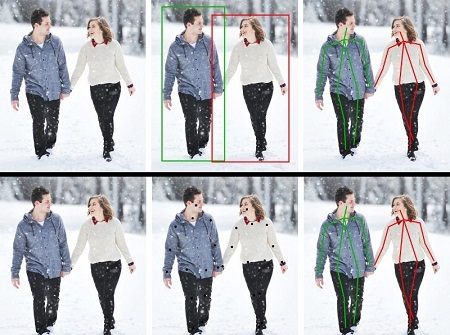
\includegraphics[scale=1.0]{bab2/gambar/tdbu.jpg}}
    \end{center}
    \vspace{-20pt}
    \captionsetup{labelfont=bf, textfont=bf}
    \caption{Pendekatan \textit{Top-Down} dan \textit{Bottom-Up}}
    \vspace{-10pt}
    \captionsetup{labelfont=md, textfont=md}
    \caption*{Sumber: https://mc.ai/an-overview-of-human-pose-estimation-with-deep-learning}
    % \caption*{Sumber: Zhang (2019)}
    \label{fig:tdbu}
\end{figure}

\section{Estimasi Pose Tiga Dimensi}
\label{sec:2-EstimasiPoseTigaDimensi}

Algoritma estimasi pose tiga dimensi merekonstruksi titik kunci tiga dimensi tubuh manusia dari
sebuah gambar dua dimensi. Proses pencarian titik kunci dibagi menjadi dua golongan yaitu pencarian
secara langsung menggunakan gambar sebagai masukkan dan pencarian bertahap dengan mencari titik kunci
anatomi dua dimensi terlebih dahulu kemudian dilanjutkan dengan pencarian titik kunci tiga dimensi.
Titik kunci yang didapatkan dapat berada dalam koordinat lokal dan global.
Pencarian secara langsung tidak menghasilkan akurasi yang tinggi dan cenderung buruk dalam mendeteksi
orientasi yang benar~\cite{2020arXiv200210322C}.

Titik kunci tiga dimensi yang berada dalam koordinat lokal menjadikan posisi pinggang sebagai titik
nol yang berarti lokasi pinggang akan selalu bernilai $\vec{hip} = [0.0, 0.0, 0.0]$. Posisi titik
kunci lain relatif terhadap titik pinggang. Hal ini menyebabkan pose yang ditangkap hanya bersifat
lokal yang berarti hanya memiliki satu orientasi lokal. Pencarian pose tiga dimensi lokal dari gambar
dua dimensi diilustrasikan pada gambar~\ref{fig:lokal}~\cite{martinez_2017_3dbaseline}.

\begin{figure}[htbp]
    \begin{center}
        \fbox{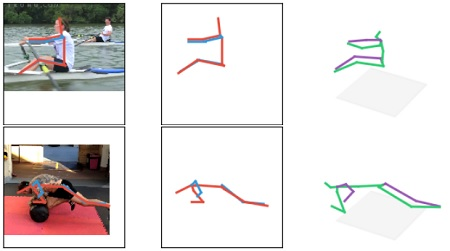
\includegraphics[scale=1.0]{bab2/gambar/lokal.jpg}}
    \end{center}
    \vspace{-20pt}
    \captionsetup{labelfont=bf, textfont=bf}
    \caption{Pencarian Pose Tiga Dimensi Lokal}
    \vspace{-10pt}
    \captionsetup{labelfont=md, textfont=md}
    \caption*{Sumber: https://arxiv.org/abs/1705.03098}
    % \caption*{Sumber: Zhang (2019)}
    \label{fig:lokal}
\end{figure}

Titik kunci tiga dimensi dapat juga berada dalam koordinat global yang berarti orientasi kamera
saat mengambil gambar diperhitungkan sebagai sebuah observasi virtual. Kompleksitas yang dihadapi
berkaitan dengan orientasi kamera yang berubah. Estimasi pose tiga dimensi global umumnya dilakukan
dengan mendeteksi titik kunci anatomi tubuh manusia ke dalam suatu dunia virtual tiga dimensi sehingga
dapat diamati dari berbagai sudut yang berkorelasi dengan kamera~\cite{2017arXiv170402447Z, 2019arXiv190700837M}.
Pencarian pose tiga dimensi global dari gambar dua dimensi diilustrasikan pada gambar~\ref{fig:global}.

\begin{figure}[htbp]
    \begin{center}
        \fbox{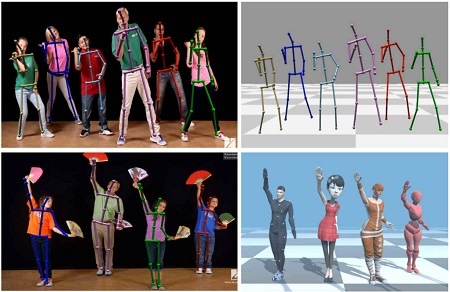
\includegraphics[scale=1.0]{bab2/gambar/global.jpg}}
    \end{center}
    \vspace{-20pt}
    \captionsetup{labelfont=bf, textfont=bf}
    \caption{Pencarian Pose Tiga Dimensi Global}
    \vspace{-10pt}
    \captionsetup{labelfont=md, textfont=md}
    \caption*{Sumber: http://gvv.mpi-inf.mpg.de/projects/SingleShotMultiPerson}
    % \caption*{Sumber: Zhang (2019)}
    \label{fig:global}
\end{figure}

\section{PyTorch}
\label{sec:2-PyTorch}

PyTorch merupakan \textit{framework} untuk melakukan \textit{deep learning} dengan bahasa pemrograman
python. Penggiat data umumnya menggunakan bahasa pemrograman ini dalam melakukan
riset pemanfaatan dan pengolahan data. PyTorch menyediakan implementasi grafik jaringan saraf tiruan yang bersifat dinamis.
Hal ini memungkinkan pengguna untuk mengubah arsitektur model secara cepat dalam setiap iterasi~\cite{2019arXiv191201703P}.


\section{\textit{Unified Modeling Language}}
\label{sec:2-uml}

\textit{Unified Modeling Language} (UML) merupakan bahasa pemodelan standar yang memiliki sintaks
dan semantik. UML bukan hanya sekedar diagram, tetapi juga menceritakan konteksnya. UML
diaplikasikan dengan beberapa maksud seperti percangan perangkat lunak, sarana komunikasi antara
perangkat lunak dengan proses bisnis, penjabaran sistem secara rinci dan pendokumentasian sistem
yang ada.

Para pengembang sistem berorientasi objek menggunakan bahasa model untuk menggambarkan, membangun
dan mendokumentasikan sistem yang mereka rancang. UML memungkinkan para pengembang aplikasi untuk
bekerja sama dengan bahasa model yang sama dalam mengaplikasikan beragam sistem. UML merupakan Alat
komunikasi yang konsisten dalam mendukung para pengembang saat ini. UML menyediakan sembilan jenis
diagram yaitu : \textit{Class Diagram, Packet Diagram, Use Case Diagram, Sequence Diagram,
    Communication Diagram, Statechart Diagram, Activity Diagram, Component Diagram} dan
\textit{Deployment Diagram}.

\textit{Activity Diagram} merupakan penggabungan dari berbagai alur aktivitas dalam sistem yang sedang
dirancang, bagaimana masing-masing alur berawal, \textit{decision} yang  mungkin  terjadi dan bagaimana
mereka  berakhir. \textit{Activity Diagram} juga dapat menggambarkan proses paralel yang mungkin terjadi
pada beberapa  eksekusi.


\begin{table}[htbp]
    \captionsetup{labelfont=bf, textfont=bf}
    \caption{Simbol-Simbol \textit{Activity Diagram}}
    \label{tab:simbolactdiagram}
    \vspace{-20pt}
    \begin{center}
        \begin{tabular}{|c|c|c|c| }
            \hline
            No & Nama                       & Gambar           & Keterangan                                \\ \hline

            1. & \begin{minipage}{.1\textwidth}
                
\includegraphics[width=\linewidth]{bab2/gambar/uml/initial.jpg}
            \end{minipage} & \textit{Initial} & Bagaimana  objek  dibentuk  atau diawali. \\ \hline

            2. & \begin{minipage}{.1\textwidth}
                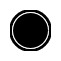
\includegraphics[width=\linewidth]{bab2/gambar/uml/final.jpg}
            \end{minipage} & \textit{Final}   & Bagaimana  objek dihancurkan.             \\ \hline

            3. & \begin{minipage}{.2\textwidth}
                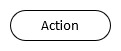
\includegraphics[width=\linewidth]{bab2/gambar/uml/action.jpg}
            \end{minipage} & \textit{Action}  & State eksekusi dari suatu aksi.           \\ \hline

            4. & \begin{minipage}{.2\textwidth}
                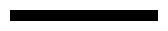
\includegraphics[width=\linewidth]{bab2/gambar/uml/fork.jpg}
            \end{minipage} & \textit{Fork}    & Penggabungan atau pemisahan alur.         \\ \hline

            5. & \begin{minipage}{.2\textwidth}
                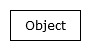
\includegraphics[width=\linewidth]{bab2/gambar/uml/object.jpg}
            \end{minipage} & \textit{Object}  & State hasil dari suatu aksi.              \\ \hline

            6. & \begin{minipage}{.2\textwidth}
                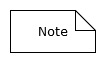
\includegraphics[width=\linewidth]{bab2/gambar/uml/note.jpg}
            \end{minipage} & \textit{Note}    & Keterangan tambahan suatu komponen.       \\ \hline
        \end{tabular}
    \end{center}
\end{table}